\documentclass[orivec]{llncs}
\usepackage{graphicx}
\usepackage{amsmath}			% for "cases"
\usepackage{amsfonts}		% for frakur fonts
\usepackage{mathrsfs}		% for curly "E" error symbol
\usepackage{float}
\usepackage[most]{tcolorbox}	% for wrapping example in color box
% \usepackage{wrapfig}			% wrap figure beside text, used in example
\usepackage{tikz-cd}			% commutative diagrams
\usepackage{tikz}
\usepackage{amssymb}			% for \multimap \updownarrow \bigstar \varnothing
\usepackage{sectsty}			% change section color
% \usepackage{turnstile}		% longer turnstiles
\usepackage{wasysym}			% smileys
\usepackage[normalem]{ulem}	% underline with line breaks: /uline
\usepackage{hyperref}		% refs, links become clickable
\usepackage[]{algorithm2e}	% algorithms

\usepackage{geometry}		% change paper size
\geometry{
  a4paper,         % or letterpaper
  textwidth=18cm,  % llncs has 12.2cm
  textheight=27cm, % llncs has 19.3cm
  heightrounded,   % integer number of lines
  hratio=1:1,      % horizontally centered
  vratio=2:3,      % not vertically centered
}
\usepackage[fontsize=13pt]{scrextend}

% *************** Delete when not using Chinese or colors **********************
\usepackage{xeCJK}
\setCJKmainfont[BoldFont=SimHei,ItalicFont=KaiTi]{SimSun}
\usepackage{color}
\definecolor{cerulean}{RGB}{100,100,200}
%\newcommand{\emp}[1]{\textbf{\textcolor{Cerulean}{#1}}}
\newcommand{\emp}[1]{\textbf{#1}}
\definecolor{grey}{rgb}{0.9,0.9,0.9}  % grey

% \chapterfont{\color{blue}}  % sets colour of chapters
\sectionfont{\color{blue}} 
\subsectionfont{\color{blue}} 
\subsubsectionfont{\color{blue}} 
\setcounter{secnumdepth}{3}		% use numbers in subsubsections

\let\emptyset\varnothing			% more beautiful empty set symbol
\newcommand{\vect}[1]{\boldsymbol{#1}}
\newcommand*\sigmoid{\vcenter{\hbox{
\includegraphics{sigmoid.png}}}}
\newcommand*\KB{\vcenter{\hbox{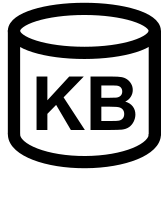
\includegraphics{KB-symbol.png}}}}
\newcommand*\NN{\vcenter{\hbox{\includegraphics{NN-symbol.png}}}}
\newcommand*\invsigmoid{\vcenter{\hbox{\includegraphics{inverse-sigmoid.png}}}}
\newcommand{\invW}{\, \rotatebox[origin=c]{90}{W}}
\newcommand{\invw}{\, \rotatebox[origin=c]{90}{w}}
\newcommand*\rectifier{\vcenter{\hbox{\includegraphics{rectifier.png}}}}
\newcommand{\dashh}{\textemdash~}
\newcommand{\tab}{\hspace*{1cm}}

\newcommand{\tikzmark}[1]{\tikz[overlay,remember picture] \node (#1) {};}

\let\labelitemi\labelitemii

\renewcommand{\thefootnote}{\fnsymbol{footnote}}
\interfootnotelinepenalty=10000

% ***** Boxed variables inside math equations
% \newcommand*{\boxedcolor}{black}
\makeatletter
% \renewcommand{\boxed}[1]{\textcolor{\boxedcolor}{%
% \fbox{\normalcolor\m@th$\displaystyle#1$}}}
% \setlength{\fboxsep}{1pt}
\renewcommand{\boxed}[1]{\fbox{\m@th$\displaystyle\scalebox{0.9}{#1}$} \,}
\makeatother

\overfullrule=0mm

\newsavebox{\MyName}
\savebox{\MyName}{
\includegraphics[scale=0.6]{YKY.png}}

\title{什么是贝叶斯网络? (What are Bayesian networks?)}
\titlerunning{什么是贝叶斯网络?}
\author{\usebox{\MyName} (King-Yin Yan)
% \\ \footnotesize{General.Intelligence@Gmail.com}
}
\institute{General.Intelligence@Gmail.com}

\begin{document}

\maketitle
\setlength{\parindent}{0em}
% \setlength{\parskip}{2.8ex plus0.8ex minus0.8ex}
\setlength{\parskip}{2.8ex}

%\begin{abstract}
%\end{abstract}

\section{命题和它们之间的关系}

上次介绍过「命题逻辑」,\textbf{命题} 即是能赋予 \textbf{真假值} (truth value) 的东西。  例如「昨天下雨」、「人是动物」等。

命题之间有「关系 relations」,例如:「吃了不洁食物」$\rightarrow$「肚子痛」; \\
记作 P $\rightarrow$ Q 或叫「P 蕴涵 Q」。

这个「\textbf{箭头}」是一切逻辑中最重要的,有了它才可以有「\textbf{推导} deduction」这回事,否则知识变成一堆离散的没关连的点子。

宇宙无限,但人脑有限,以有限的脑怎能理解无限的世界? 那是靠 general rules。  那些 rules 里面有变量 (variables),所以逻辑 formulas 可以像 template (模版) 那样套到不同的实例上,然后推出不同的结论,於是「经验世界」可以被\textbf{压缩}成有限的资讯。

总言之,\textbf{变量}是\textbf{压缩}的基础,\textbf{箭头}是\textbf{推导}的基础。

\section{机率}

但,在经典逻辑中,所有命题都是 \textbf{非真即假} (binary)的,这当然有局限,所以我们这一代的研究者都不用经典逻辑了。   我的 Genifer、Ben Goertzel 的 OpenCog、王培的 OpenNARS,我们都设计了某种 ``uncertainty logic''。 
\begin{equation}
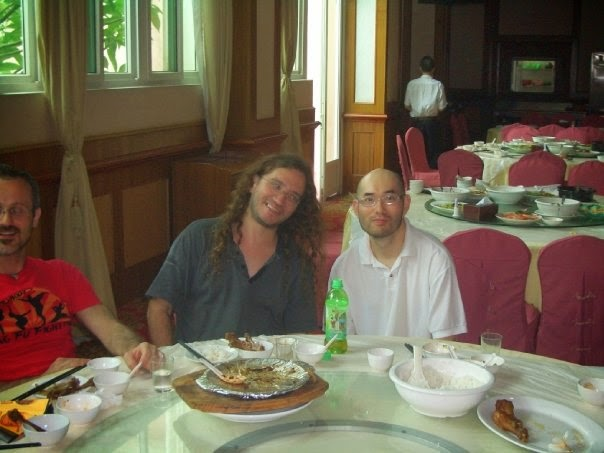
\includegraphics[scale=0.4]{YKY-and-BenGoertzel.jpg}
\quad
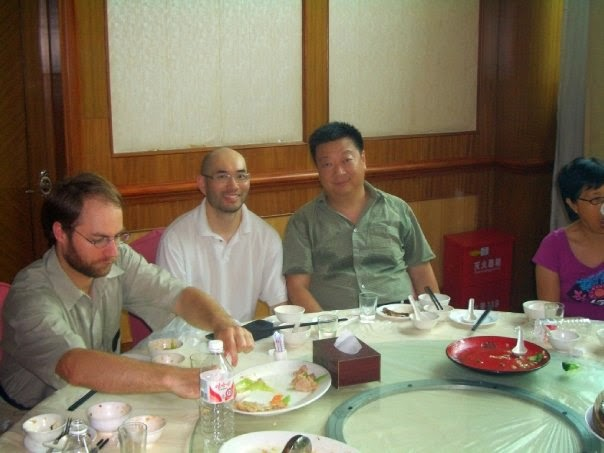
\includegraphics[scale=0.4]{YKY-and-PeiWang.jpg}
\nonumber
\end{equation}

我使用的办法是经典的概率论加上模糊性 (fuzzy);  例如,如果说「玛莉很高」,那概率的分布就可以像下图的红色曲线那样:
\begin{equation}
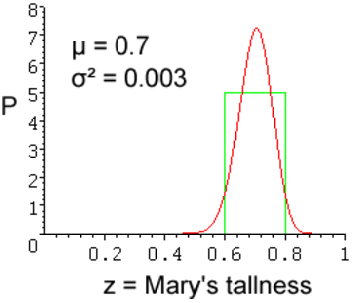
\includegraphics[scale=0.8]{P-over-Z-Marys-Tallness2.png}
\end{equation}
即是说,玛莉的高度,是以不确定的概率分布,而最有可能的高度就是尖端的 peak 位置。  注意,我不标示真正的高度,而是用 [0,1] 这区间来表示「高」的程度,例如 0.7 是比平均高的, 0.5 则是平均。

但如果不确定性增加的话,那曲线会变得更扁,例如:
\begin{equation}
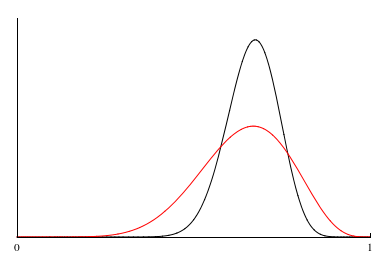
\includegraphics[scale=0.65]{PZ-broad-and-narrow.png}
\end{equation}

还有,机率的特性,就是它分布的曲线下面的总面积一定是 1,因为无论玛莉的高度如何分布,所有可能性的总和就是一个「必然事件」,而必然事件的机率是1。 

\begin{equation}
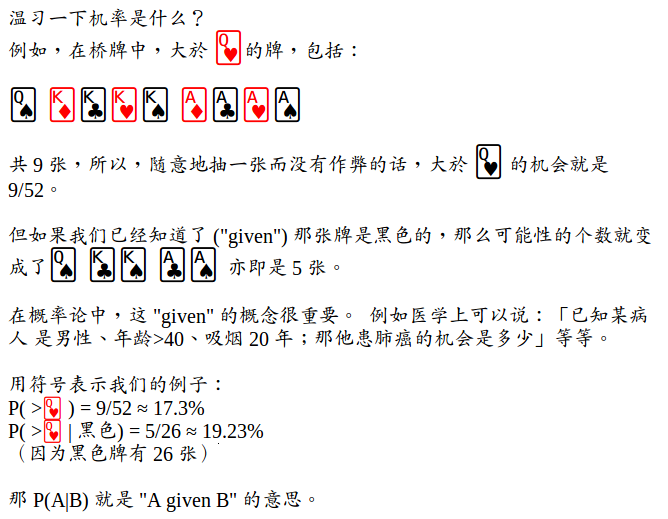
\includegraphics[scale=0.75]{probabilities-refresh.png}
\end{equation}

\section{Bayesian network}

以下是一个 Bayesian network 的例子 :
\begin{equation}
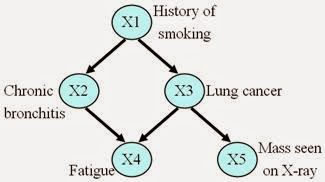
\includegraphics[scale=0.8]{Bayes-net-example.jpg}
\end{equation}
每一个箭头,如果是由 X 指向 Y,便表示 ``Y given X'',亦即是「如果知道了 X 发生的话,Y 的机会是多少」。

例如在图中可看到,吸烟影响肺癌、肺癌影响疲倦、肺癌也影响 X-ray 的结果。

在上图中每个箭头,都附带有一些 $P(X|Y)$ 那样的数据,如下表所示:\\
(不需深究)
\begin{equation}
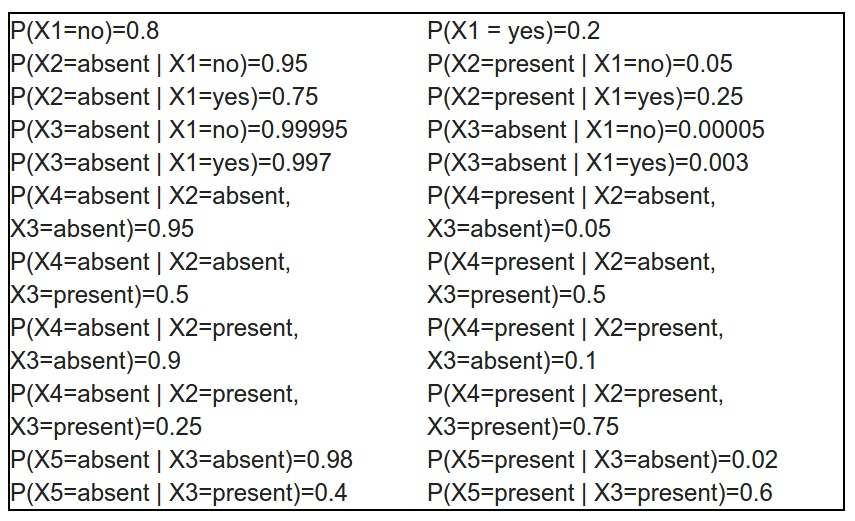
\includegraphics[scale=0.4]{conditional-probability-table.jpg}
\end{equation}

之所以叫 Bayesian network,是因为 Thomas Bayes 这个和牛顿同期的数学家:
\begin{equation}
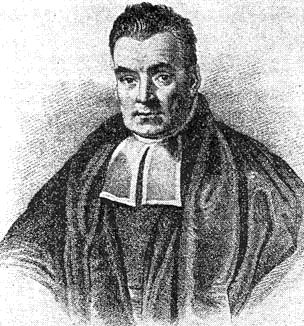
\includegraphics[scale=0.6]{Thomas-Bayes.png}
\end{equation}
他发现了一个公式可以用来计算 $P(X|Y)$ 那样的机率 :
\begin{equation}
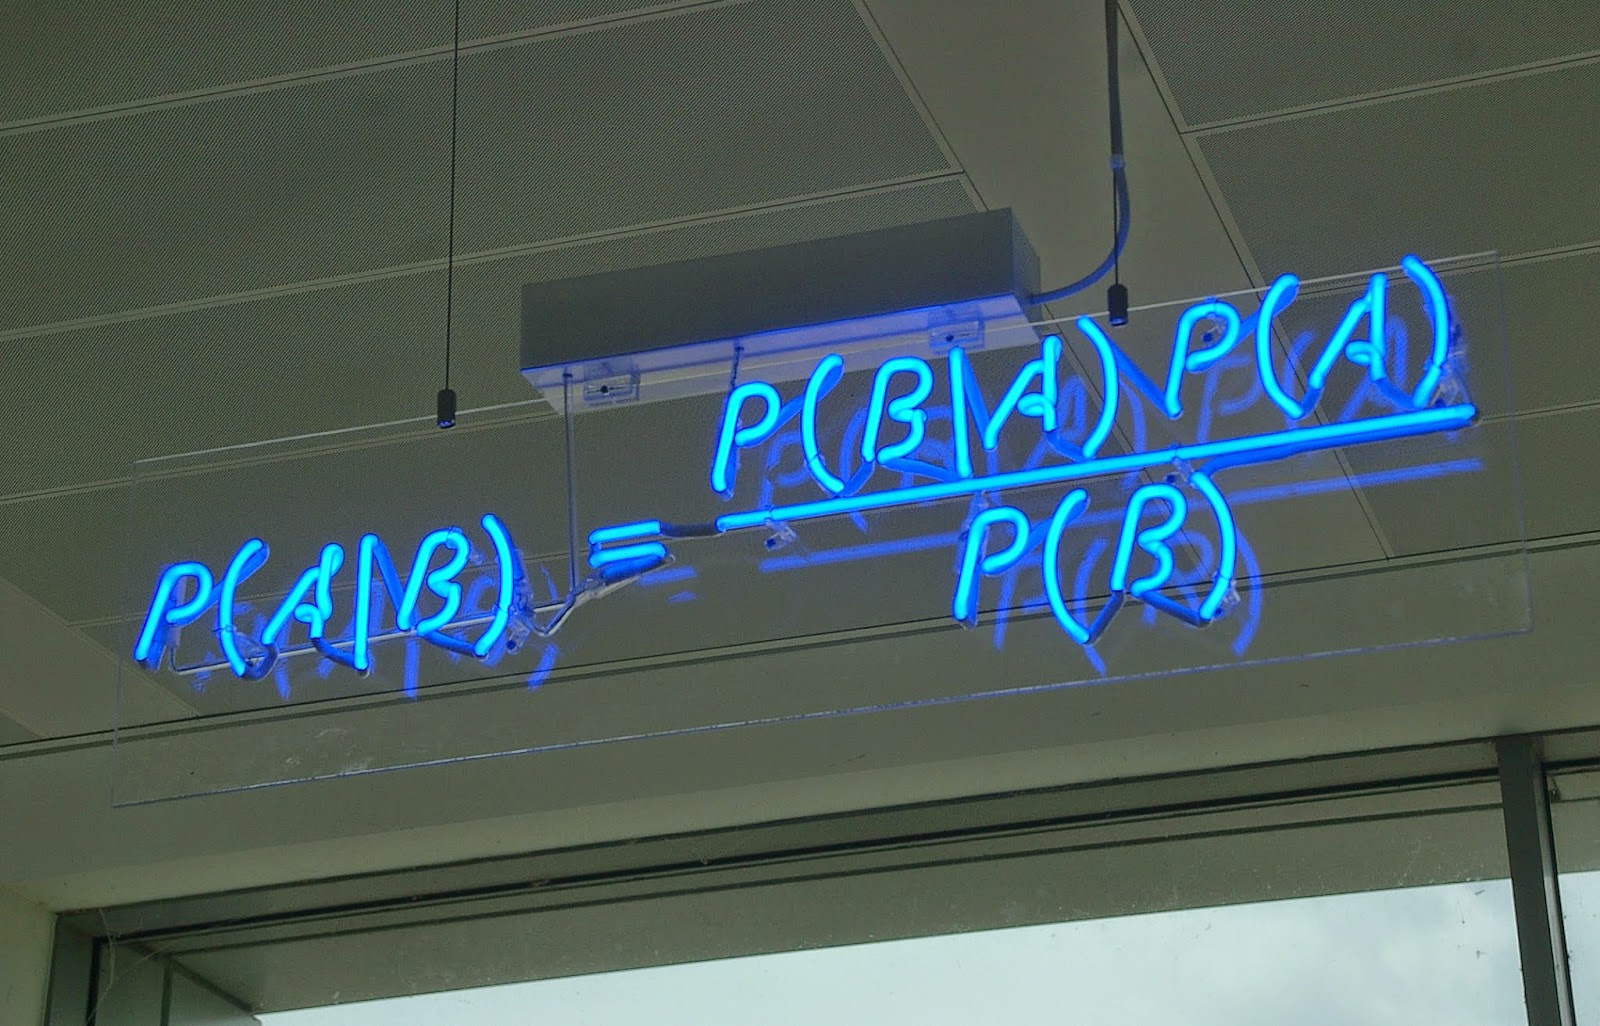
\includegraphics[scale=0.25]{Bayes-Theorem-(sign).jpg}
\end{equation}

亦可以更为对称地写成:
\begin{equation}
P(A|B)P(B) = P(A,B) = P(B|A)P(A)
\end{equation}
其中 $P(A,B)$ 是 "A and B" 都发生的机率,和 "A given B" 不同。

这公式在初中或高中会学到,不是很难明。

贝叶斯网络的难处,是在於网络把不同的机率连系起来了,所以 Bayes rule 要一个套着一个地连续运用,变成很复杂、很多 sum of products。  但其实如果有耐性和细心的话,那个算法应该不难,因为除了 Bayes rule 与及机率的基本运算之外, 就没有其他了。 

\section{参考资料}

以前经典 AI 不用机率,直到 1980's Judea Pearl 写了一本很详细分析 Bayesian network 的书,使它变成主流:
\begin{equation}
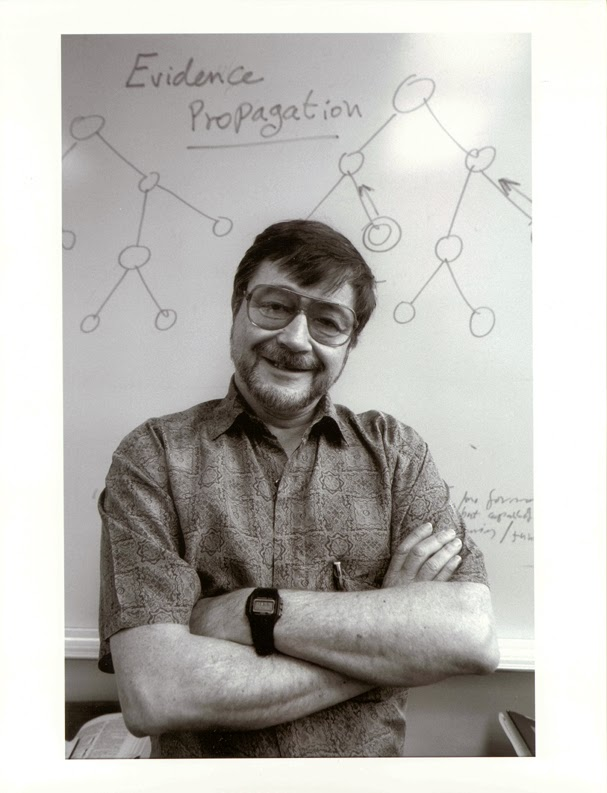
\includegraphics[scale=0.4]{Judea-Pearl.jpg}
\quad
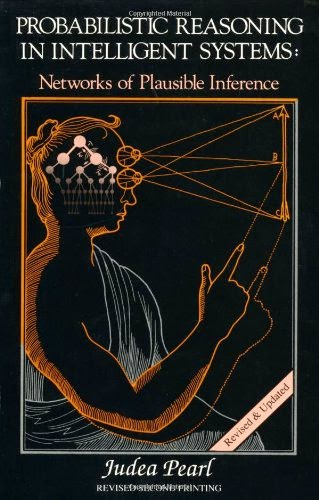
\includegraphics[scale=0.5]{Pearl-book-cover.jpg}
\nonumber
\end{equation}
Pearl 的儿子是美国驻伊拉克记者,他们家是犹太人,他不幸被恐怖分子捉了而被割首,过程被摄影下来。  我不能断定他是极端亲美,还是作为一个同情者而被无辜杀害 ?

另外这个是 Daphne Koller,她是这本新的巨著 (2009 年,1280 pages!) 的作者之一:
\begin{equation}
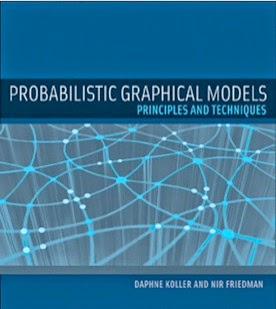
\includegraphics[scale=0.6]{Koller-book-cover.jpg}
\quad
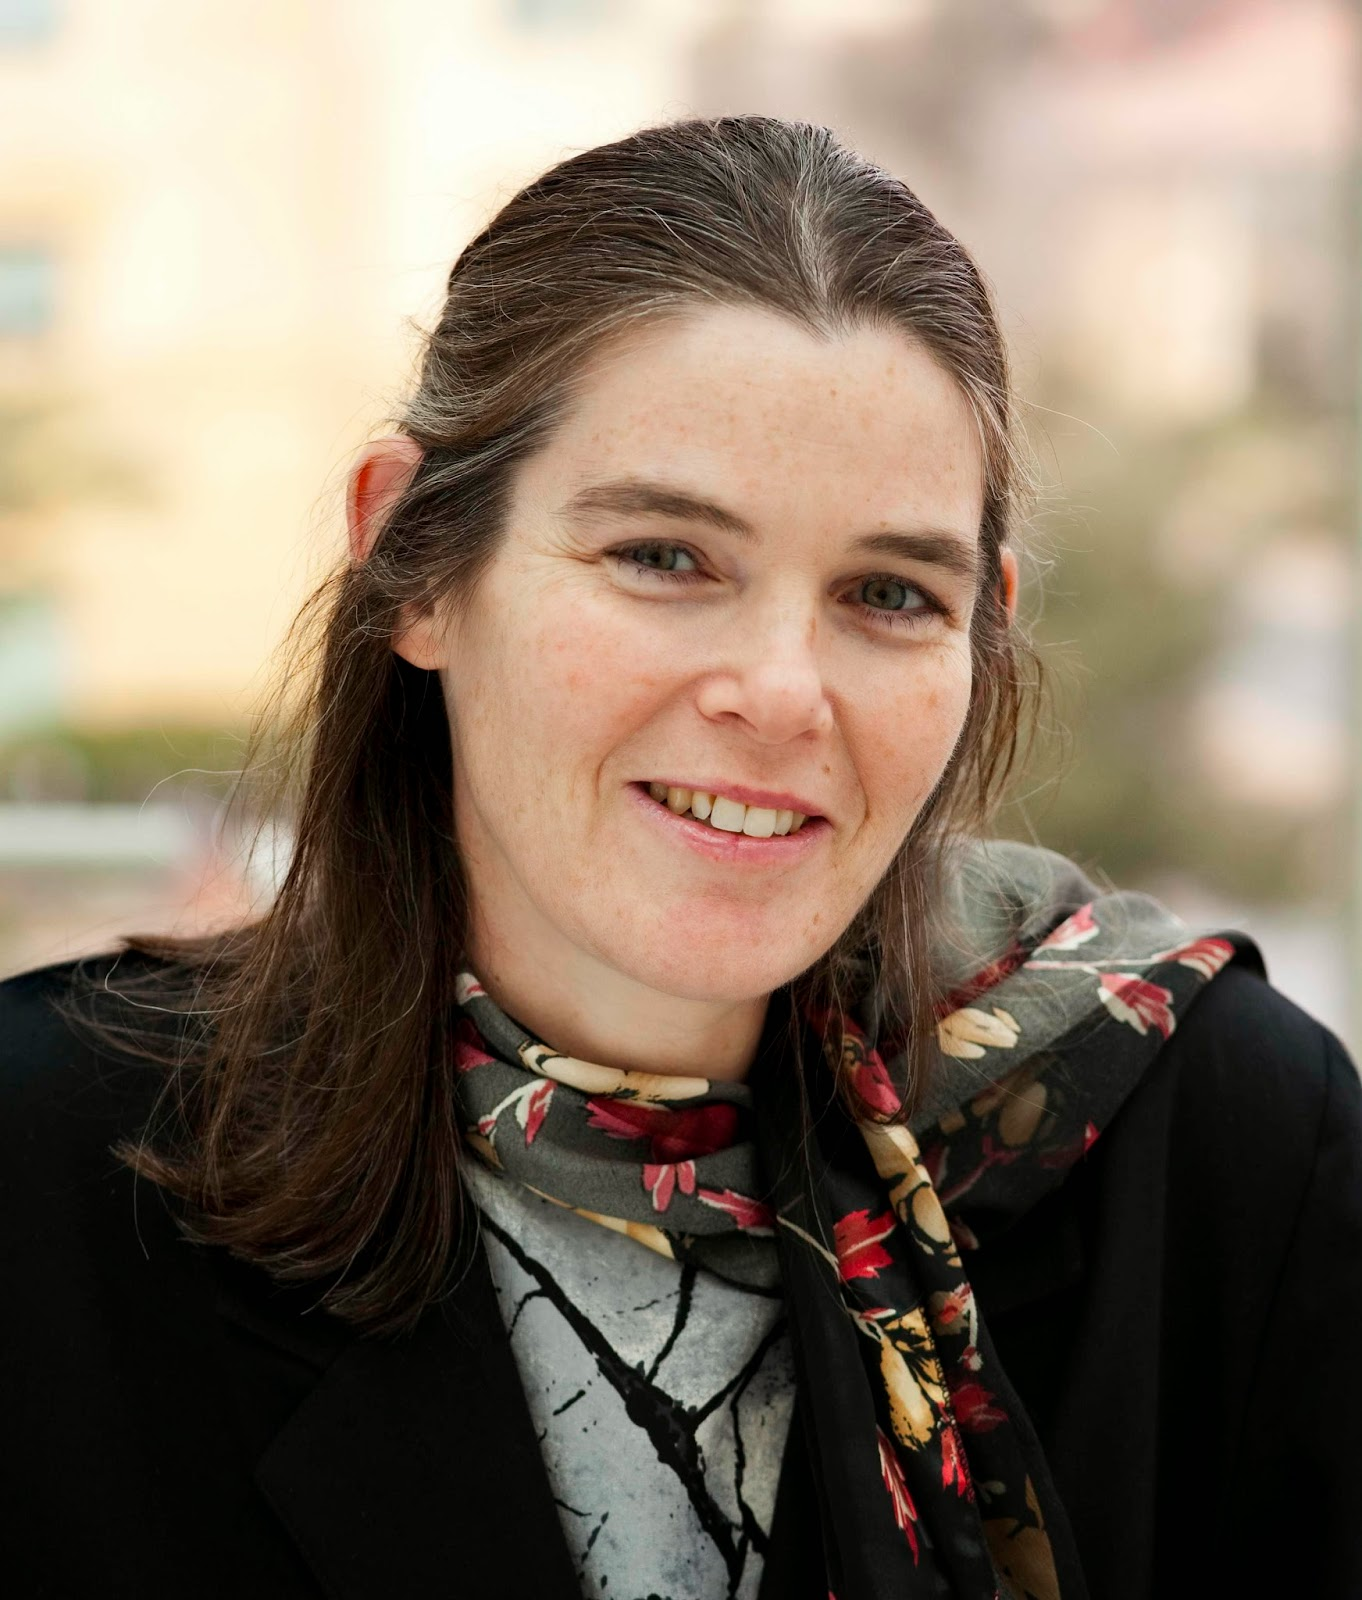
\includegraphics[scale=0.15]{daphne2011.jpg}
\nonumber
\end{equation}
但这本书太 technical 和详细,对初学者不好读。

在 Stanford U 的 Daphne 是 Coursera 的创始人之一,她的(免费的)课 \url{https://www.coursera.org/course/pgm} 详细地讲解 Bayesian network 的算法和学习法。  

顺带一提,这个是 Peter Norvig,他和 Stewart Russell 合著的 "AIMA" 是现时最好的人工智能教科书。
\begin{equation}
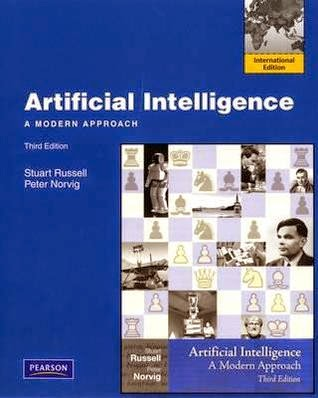
\includegraphics[scale=0.5]{AIMA-book-cover.jpg}
\quad
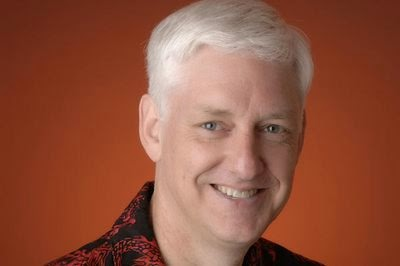
\includegraphics[scale=0.6]{Norvig.jpg}
\nonumber
\end{equation}

\quad \quad \quad --- 完 ---

%\bibliographystyle{plain} % or number or aaai ...
%\bibliography{AGI-book}

\end{document}
